\chapter{トランスポート層(その3) TCP}


TCP(Transport Controll Protocol)は、インターネットプロトコルスイートにおいて、アプリケーション層に対して、確実な通信を提供するためのトランスポート層プロトコルです。この確実な通信を行うために、複雑な手順を経て通信を行っています。この章では、TCPが、確実な通信のために何をしているかを説明します。

確実な通信を行うためには、データの取りこぼしを防ぐ仕組みが必要とです。それについても説明をします。本書での説明は、イメージをつかむためのごく簡単なものです。そのため、詳しく知りたい場合は、本書付録付録や参考文献を参照してくださいね。

\section{確実な通信}

TCPでは、どのようにして確実な通信を行っているのだろうか?先ほどトランスポート層の機能として簡単に説明したが、それをもう少し掘り下げてみよう。

TCPは、確実な通信を行うために、おおまかに以下のようなことを行っている。

\begin{enumerate}
\item データを受信したら、送信側に、「届いた」という連絡をする。
\item 通信の相手が通信できる状態にあることを確認しあう
\item データをどれだけ流すかは、通信相手の自己申告に従う。また、経路の状況に応じて、調整する。
\item 「届いた」という連絡がない場合は、データを送信し直す。
\item データを受信したら、送信側に、「届いた」という連絡をする
\end{enumerate}


確実な通信をおこなうために、まず、データを受信したら、送信側に、届いたという連絡を入れることにしよう。だが、TCPが使用する下位のレイヤが提供するサービス、つまりインターネットプロトコル層が提供するサービスにはそのような機能はない。そのため、インターネットプロトコル層のサービスを使って、届いたという連絡をしたり、届いたという連絡を受けたらデータの送信が成功したことを理解するのは、TCPの仕事となる。

\subsection{ストリームとセグメント}
まず、TCPのストリームとセグメントという言葉を定義しておこう。

ストリームは、アプリケーション層から渡されたデータ、あるいはアプリケーション層に渡すデータである。アプリケーション層がトランスポート層としてTCPを使用する場合は、トランスポート層以下のデータ転送単位を考慮しない。また、データをビット列と見たとき、その送信順が保存されることを期待している。

一方のセグメントは、TCPがストリームを分割して、一度に送出できるデータの大きさに切り分けたものである。セグメントが、一度に送出される、つまり、インターネットプロt凝る層に渡されるデータ量となる。

\subsection{セグメントが一つだけの場合}
\begin{wrapfigure}[22]{r}{6cm}
	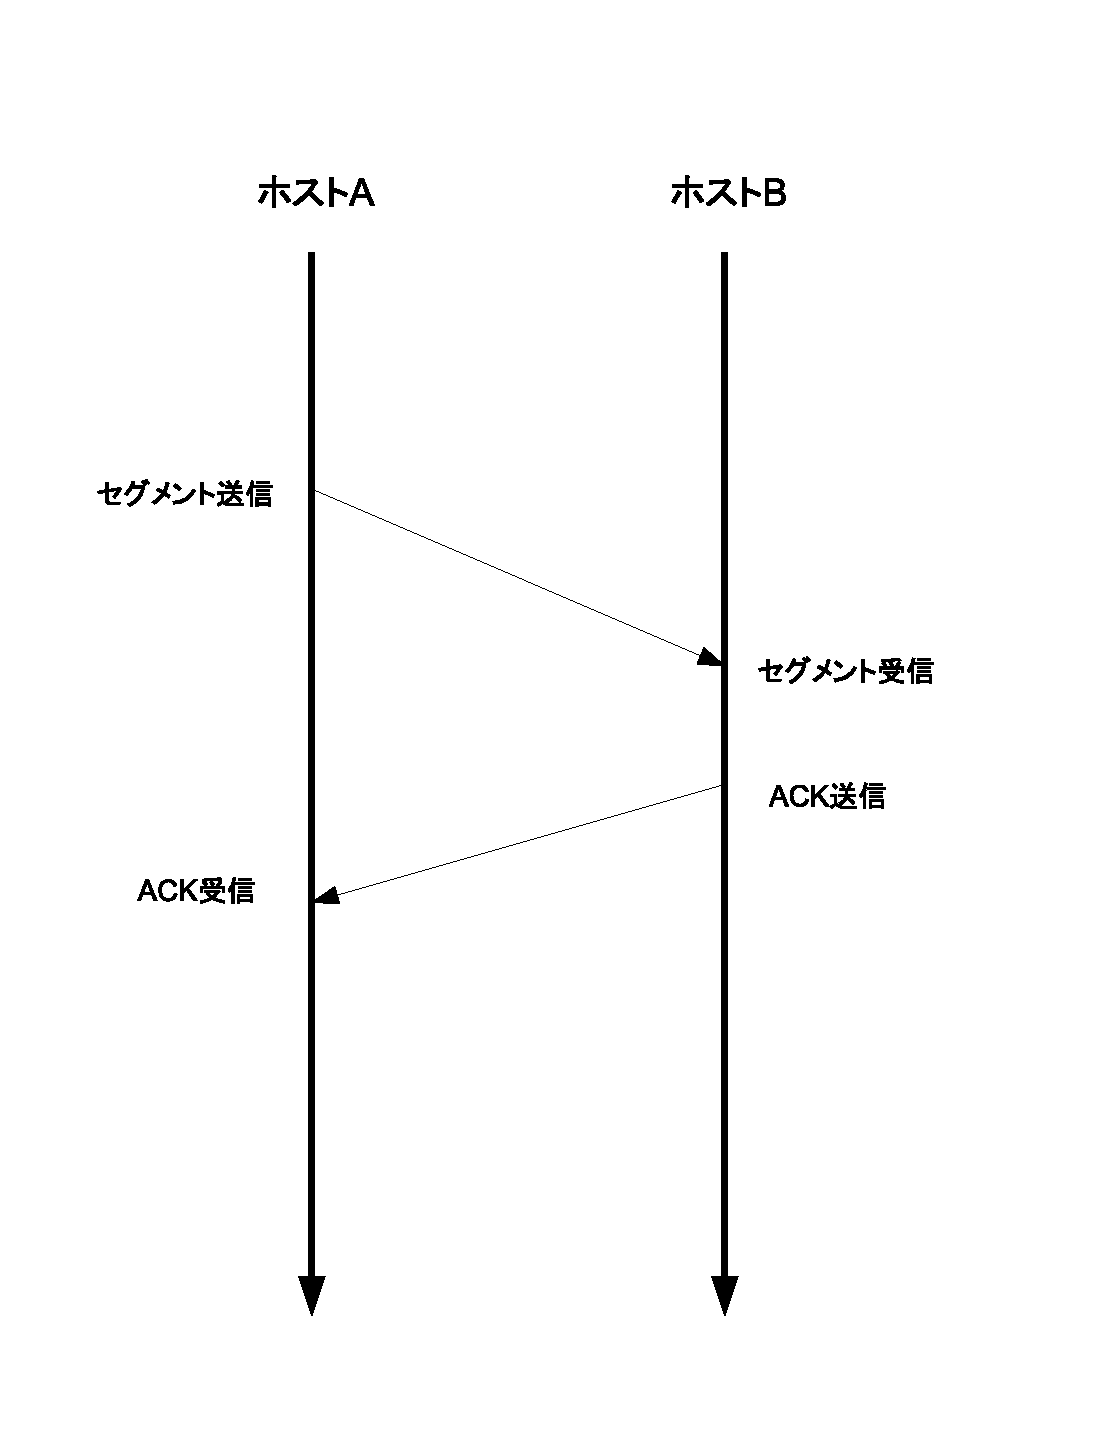
\includegraphics[width=6cm, clip]{draw/tcp01n.eps}
	\caption{セグメント一つの送信と応答}
	\label{fig:tcp01}
\end{wrapfigure}

まず、TCPで通信を行っているホストAとホストBがあるとしよう。ホストAがホストBに向けて、何らかのデータをひとつだけ送信したとする。このデータが、TCPのデータの送信単位、つまりセグメントとなる。

ホストBがセグメントを受信すると、送信元であるホストAにむけて、届いたという返事を返す。ホストAは、ホストBからの、届いたという返事を受信したら、セグメントの送信に成功したことを知ることができる。つまり、一つのセグメントの送信について、確実な通信ができたということだ。

この、届いたという返事を確認応答(ACK Acknowledgement)という。ACKは、TCPヘッダのACKビットフィールドを1にした、TCPセグメントとして送信される。

\subsection{ACKが届かない場合}

セグメントもACKも、インターネットプロトコル層によって伝送される。そのため、セグメントとACK、どちらかが届かない場合もある。では、ACKが届かない場合はどのようにすればよいのだろうか。前にも説明したとおり、送信側はセグメントが届いていないのかACKが届いていないのか、判断することができない。

そこで、ACKが届かない場合は、届くことを期待していたACKに対応するセグメントを、もう一度送信する。前に送ったセグメントがホストBにとどいていなければ、送信し直した方のセグメントが受信され、ACKが帰ってくるだろう。

では、ホストBは先に送ったセグメントを受信してACKを返していたが、そのACKがホストAに届かなかった場合はどうなるだろうか。ホストBは送信し直したセグメントを受信した後に、ホストAにACKを返す。そして、重複したセグメントを破棄する。

このように、ACKが返らない場合は、ACKが返るまで、送信側はそのACKに対応するセグメントを送信し直す。つまり、TCPの確実なやり取りとは、ACKと、ACKが届かなかったときのセグメントの送信し直しで成り立っている。

\subsection{シーケンス番号と確認応答番号}
\begin{wrapfigure}[22]{r}{6cm}
	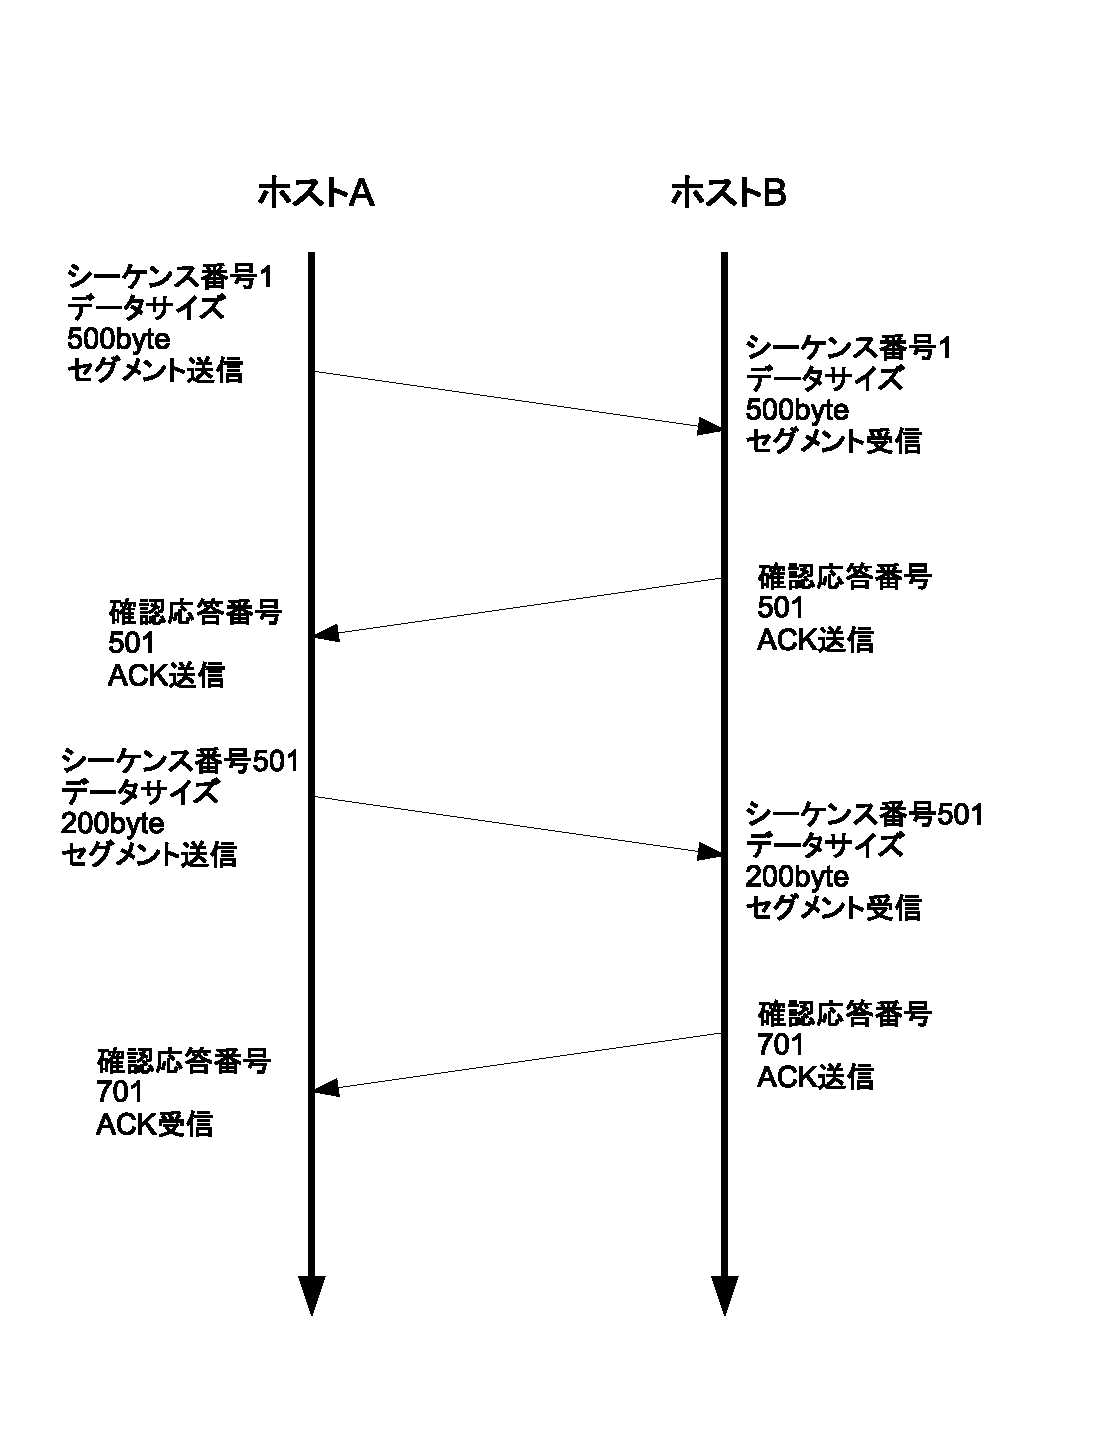
\includegraphics[width=6cm, clip]{draw/tcp02n.eps}
	\caption{シーケンス番号と確認応答}
	\label{fig:tcp02}
\end{wrapfigure}

ホストAが送信するセグメントが複数であった場合を考えよう。この場合には、セグメント一つを送信する場合にはない問題が生じる。それは、戻ってきたACKがどのセグメントに対応しているかわからないということである。

インターネットプロトコル層の特性を考えると、ホストAが送信したセグメント(をデータとして持つIPデータグラム)が、その送信順にホストBに到着する保証はない。同様に、ホストBが送出したACKが、送信した順番でホストAに到着する保証もない。さらに、セグメントのどれか、ACKのどれかが到着しない可能性もある。このとき、どのACKがどのセグメントに対してのACKかを区別するにはどのような方法があるだろうか。

どのセグメントに対するACKかを判別するために、セグメントとACKに番号を付ける。そして、セグメントの番号と、ACKの番号を対応させて、どの ACKがどのセグメントに対応しているかを判別すればよい。

セグメントに付ける番号は、シーケンス番号と呼ばれる。ここで気をつける必要があるのが、シーケンス番号はセグメントの送信順に付けられる番号ではないということだ。シーケンス番号は、そのセグメントで運ぶデータが、上位のアプリケーション層から渡されたストリームの先頭から数えて何オクテット目になるか、を示す番号である。\footnote{TCPでは、ポート番号ごとにシーケンス番号が存在する、ということである。}

説明のために例を示そう。シーケンス番号1のセグメントが、500バイトのデータを持っていたとする。すると、その次に送信されるセグメントのシーケンス番号は、501になる。ここで、シーケンス番号501のセグメントが、200バイトのデータを持っていたとしたら、その次に送信されるセグメントのシーケンス番号は、701になるであろう。

では、ACKに付けられる番号はどのように決められるのであろうか。ACKの番号とは、このACKを受信した後で、ストリームの先頭から数えて、この番号にあたるオクテットからデータを送信してほしい、という番号である。そのため、ACKの番号はシーケンス番号ではなく、確認応答番号と呼ばれる。

では、ACKにつける番号として、シーケンス番号でなく、次はここからデータを送って、という確認応答番号を使用するのはなぜだろうか。シーケンス番号をそのまま返せば、送信側はそれで確認ができるのではないだろうか。

ACKが確認応答番号を使用する理由を説明するためには、簡単にでも、送信したセグメントがどのように受信されるかを説明しなければならない。到着したセグメントのデータ部分は、受信側のバッファに入れられる。そして、シーケンス番号の順に、上位のアプリケーションに引き渡される。ここで、セグメントの到着順が前後した場合にどうなるかを考えてみよう。受信側は、まだ到着していないセグメントを受信するまで、それ以降のシーケンス番号を持ったセグメントのデータは、バッファに置かれたままとなる。このように、TCPの受信では、到着したデータが送信順にアプリケーションに引き渡されるように、バッファにデータを留め置くことがある。

確認応答番号を使用すれば、複数セグメントについてのACKを、ひとつのACKにまとめて通知をすることができる。先の例で行けば、シーケンス番号1と501の二つのセグメントが、ホストAからホストBに送信されたとする。そして、シーケンス番号501のセグメントは200バイトのデータを持っていたとしよう。このとき、受信側のホストBは、確認応答番号501と701のふたつのACKを返してもよい。また、確認応答番号701のACKを一つ返すだけでもいい。このどちらでも、送信側ホストAは、ストリームの先頭から700オクテット分のデータが受信されたことを知ることができる。

ACKでは、シーケンス番号でなく、確認応答番号を用いることで、送信しなければならないACKを減らすことができる。

\subsection{通信の相手が、通信できる状態にあることを確認しあう}
\begin{wrapfigure}[22]{r}{7cm}
	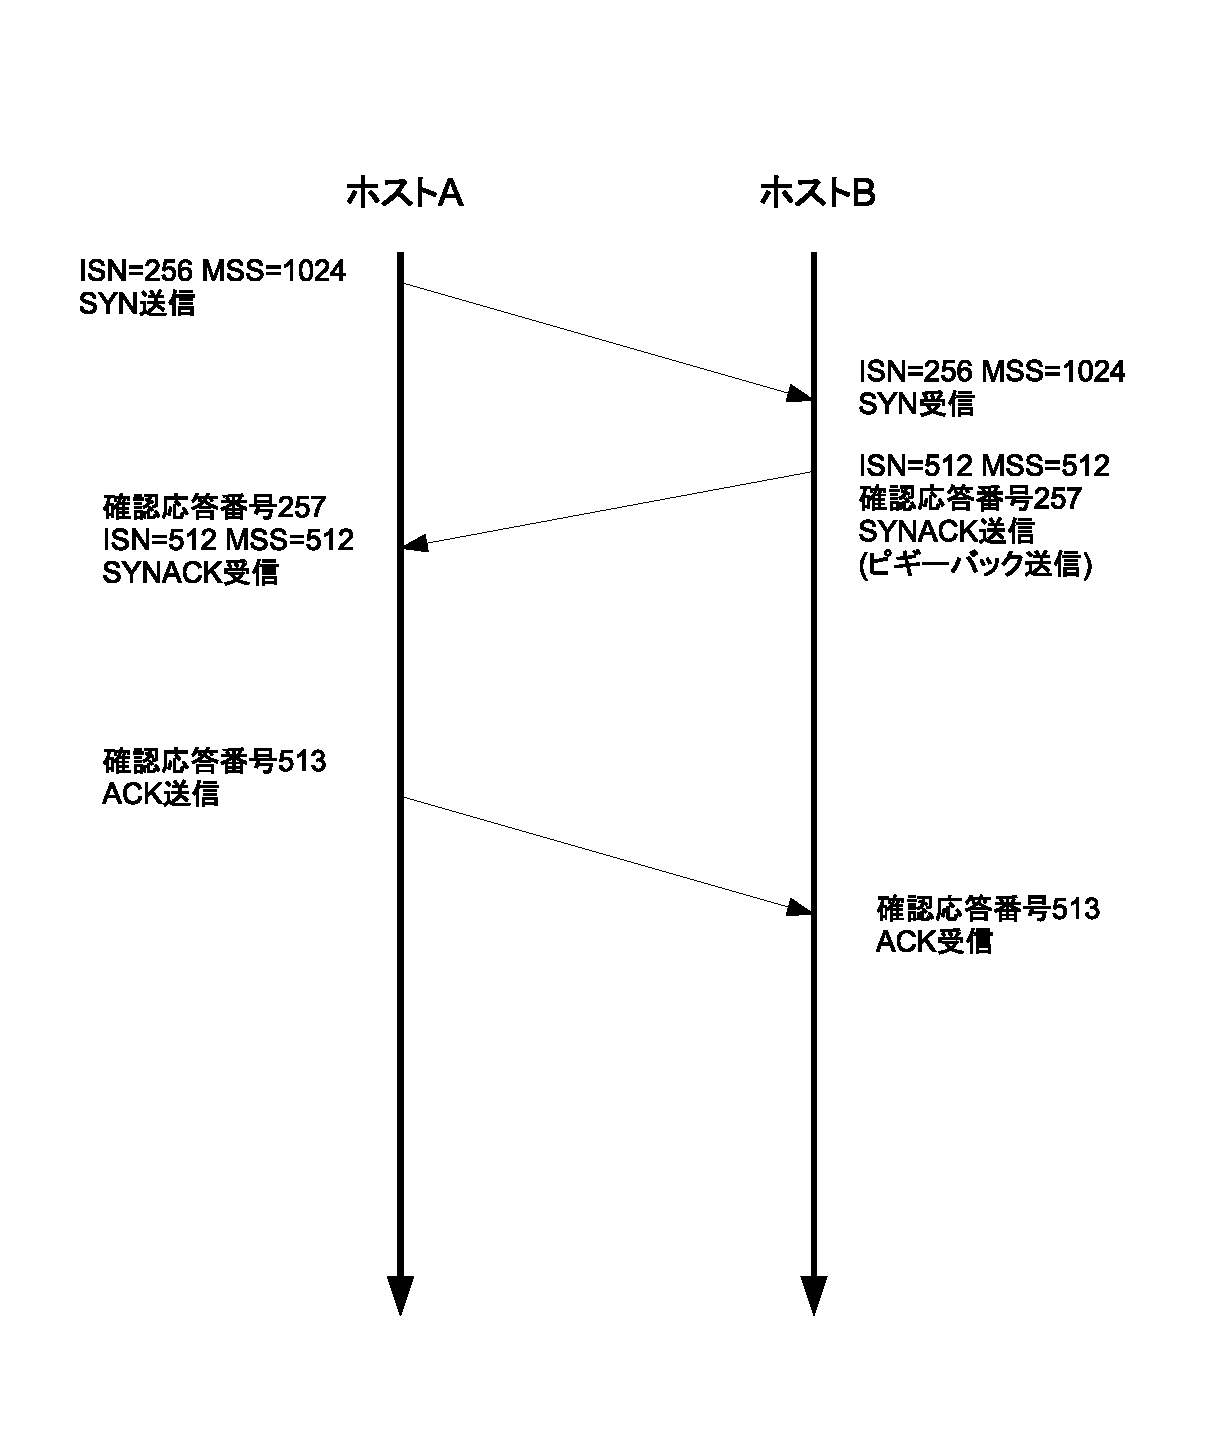
\includegraphics[width=7cm, clip]{draw/tcp04n.eps}
	\caption{3way Handshake}
	\label{fig:tcp04}
\end{wrapfigure}


TCPでは、確実な通信を行うために、通信の相手が通信できる状態にあることを確認しあう。では、TCPの説明の最初に、この手順の説明を行わなかった理由はなんだろうか。それは、TCPでは、通信の相手を確認するために、ACKを使用するためである。

ホストAからホストBに対して、TCPによる通信を開始する場合のタイムラインを追いかけてみよう。

まず、ホストAは、SYNという、これから通信を開始したい、という意味を持つセグメントをホストBにむけて送信する。この一番最初のセグメントは、UDP同様、無手順で送信される。このSYNは、TCPヘッダのSYNビットフィールドを1にした、データ部分のないセグメントである。また、SYNには、ISN(Initial Sequende Number)とMSS(Maximum Segment Size)という二つの情報が付加されている。SYNの持つこの二つの情報は何を表すのだろうか。



ISNは、ここまでで説明したシーケンス番号を、今後の通信で何番から始めるか、という値である。シーケンス番号は無符号32bit整数であり、セキュリティ上ランダムな番号をISNとすることが多い。つまり、シーケンス番号は1から始まるとは限らない。むしろ、1から始まることの方が珍しい。

MSSは、その名の通り、送信を期待するセグメントの大きさの上限である。経路のインターネットプロトコル層でフラグメントされないであろう大きさが設定される。

SYNを受け取った側は、そのSYNに対してACKを返す。ここで、ACKの返す確認応答番号は、SYNについていたISNに1を加えたものとなる。SYN はデータ部分を持たない。それなのに、なぜシーケンス番号を消費するのか。それは、ACKが送信されるときは、それが応答するするセグメントのシーケンス番号より大きい番号を、次にここから送信しろという意味で確認応答番号とする、というルールに例外をつけないため、と思えばよいだろう。

次に、ホストBは、ホストAにむけてSYNを送る。このとき、ホストB側のISNとMSSの情報を、SYNに乗せる。

このホストBから続けて送られるACKとSYNは、通常は分けて送らない。同じTCPのヘッダで、SYNとACKの両方のフラグを立てて送信する。そのため、ホストBから、応答としてSYNACKを返す、という表現をする。

SYNACKは、TCPヘッダのSYNビットフィールドとACKビットフィールドが1であり、シーケンス番号のフィールドにISN、確認応答番号のフィールドに、ホストAのSYNのISNに対する確認応答番号番号が入った、TCPセグメントとなる。

最後にホストAが、ホストBからのSYNに対するACKを返す。これで、お互いに通信ができる状態にあることを確認する手続きが完了した。ここまで完了したとき、ホストAとホストBの間で、コネクションが確立した、という。

コネクションが確立したときに、最初にSYNを送信した側をアクティブオープン、それに応答してSYNACKを返した側を、パッシブオープンという。

また、コネクションが確立するまで、ホストAからBへ(SYN)、ホストBからAへ(SYNACK)、ホストAからBへ(ACK)と、3回、セグメントが送受信される。そのため、TCPのコネクション確立を、3way Handshakeという。

TCPのコネクション確立に限ったことではないが、中央集権的な「交換機」に相当するものがないネットワークでは、全てのエンドは対等な地位にある。コネクションは、通信を行うこと必要になったエンドが、通信相手にコネクションの開設を要求することで行われる。この、コネクションを要求する側をイニシエイター、良い宇窮される側をターゲットと呼ぶことがある。\footnote{SANの一種であるiSCSIも、イニシエイター、ターゲットという用語を用いる。}


\subsection{通信を切断する}
コネクションを確立する手順が存在したのだから、コネクションを切断する手順も存在する。

まず、何をもってコネクション切断というのかを定義しよう。それは、通信を行っている双方が、相手からこれ以上送信されるデータはないという事を確認しあった状態であるとする。

\begin{wrapfigure}[21]{r}{7cm}
	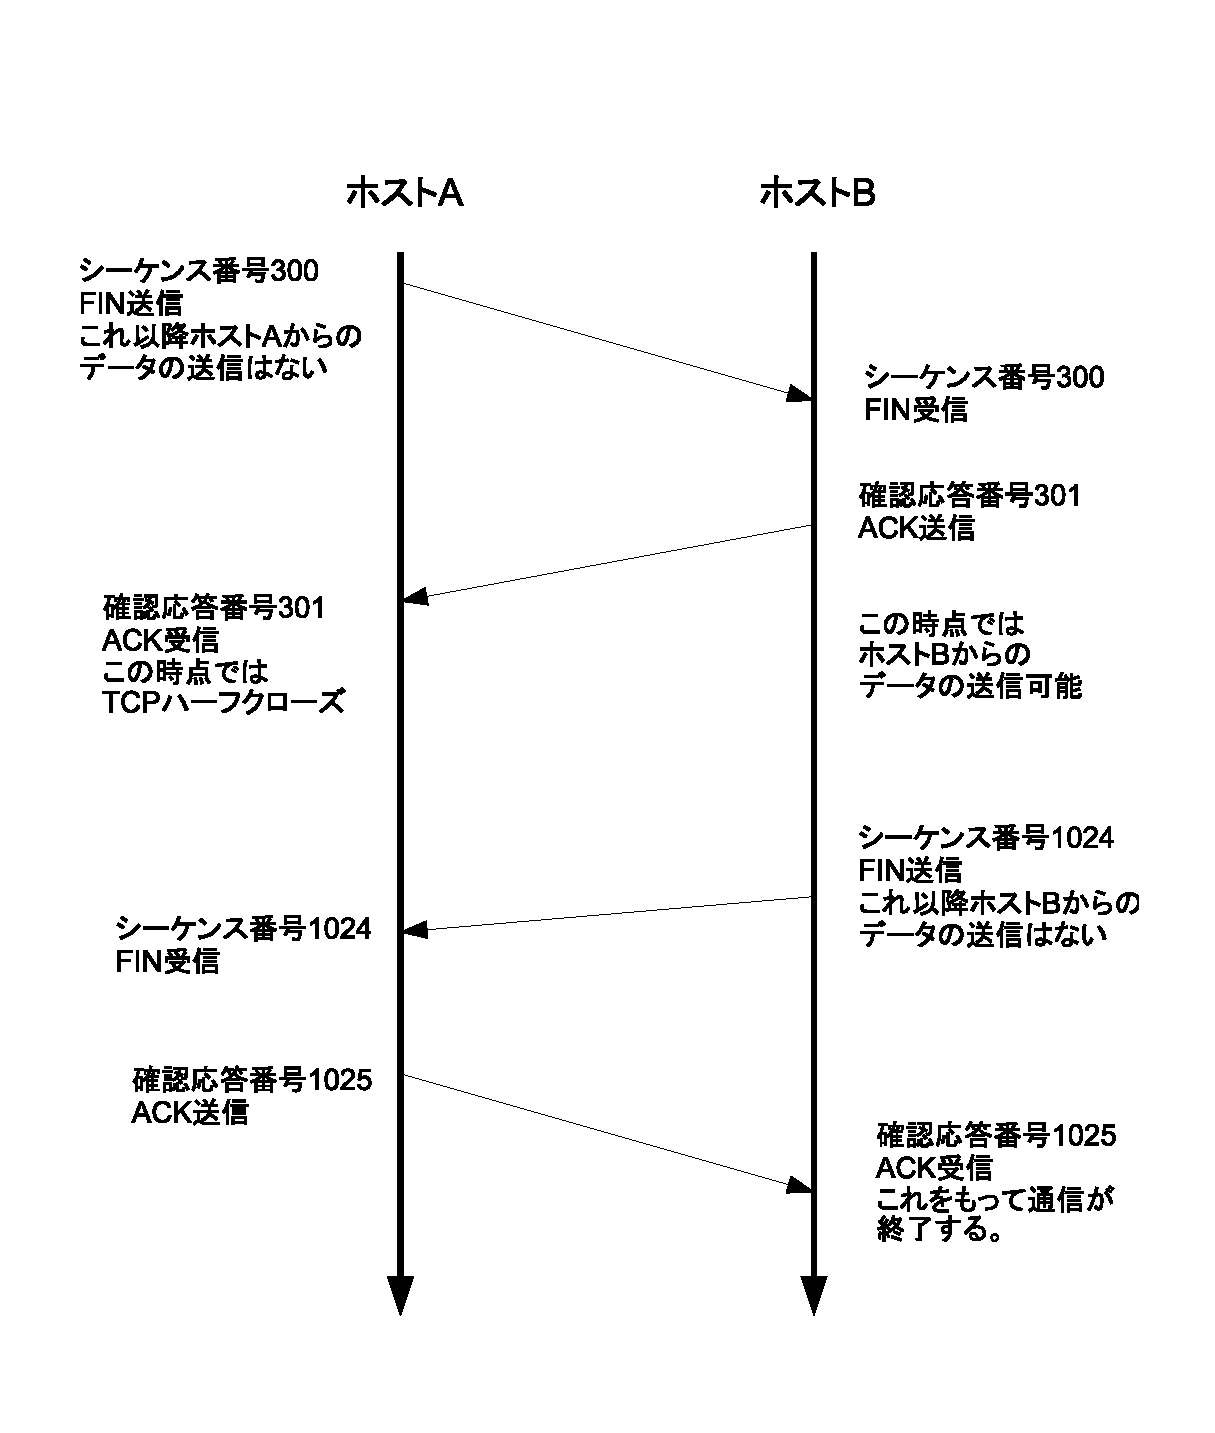
\includegraphics[width=7cm, clip]{draw/tcp05n.eps}
	\caption{コネクション切断}
	\label{fig:tcp05}
\end{wrapfigure}

例として、ホストAとホストBがコネクションを確立し、通信していたとしよう。ここで、ホストAからの、全てのデータの送信が終了したとする。このとき、ホストAは、ホストBにむかって、FINというセグメントを送信する。FINは、TCPヘッダのFINビットフィールドが1 であり、シーケンス番号を持つTCPセグメントである。このホストAからのFINを受信したホストBは、そのFINに対してのACKを返す。

だが、このホストBが出すACKは、ホストBからのFINに乗せる、いわばFINACKとして送信されることはない。それはなぜだろう。

それは、ホストAからFINが到着した時点では、ホストAから送信されるデータはもうないという意味であり、即時のコネクション切断を求めるという意味ではないためである。そのため。ホストAからFINを受け取った後でも、ホストBからホストAに向けてデータを送信することが可能である。このように、通信を行っている片方からFINが来て、それにACKを返した後に、FINを送信した側へデータを送る状態を、TCPハーフクローズという。

TCPハーフクローズの状態でも、ホストBから送信されるセグメントに対して、ホストAはACKを返す。この状態では、このコネクションにおいて、ホストAからデータが送信されることがなくなっただけである。ホストAがホストBから送信されるセグメントの受信が終了したわけではない。

\begin{wrapfigure}[15]{r}{6cm}
	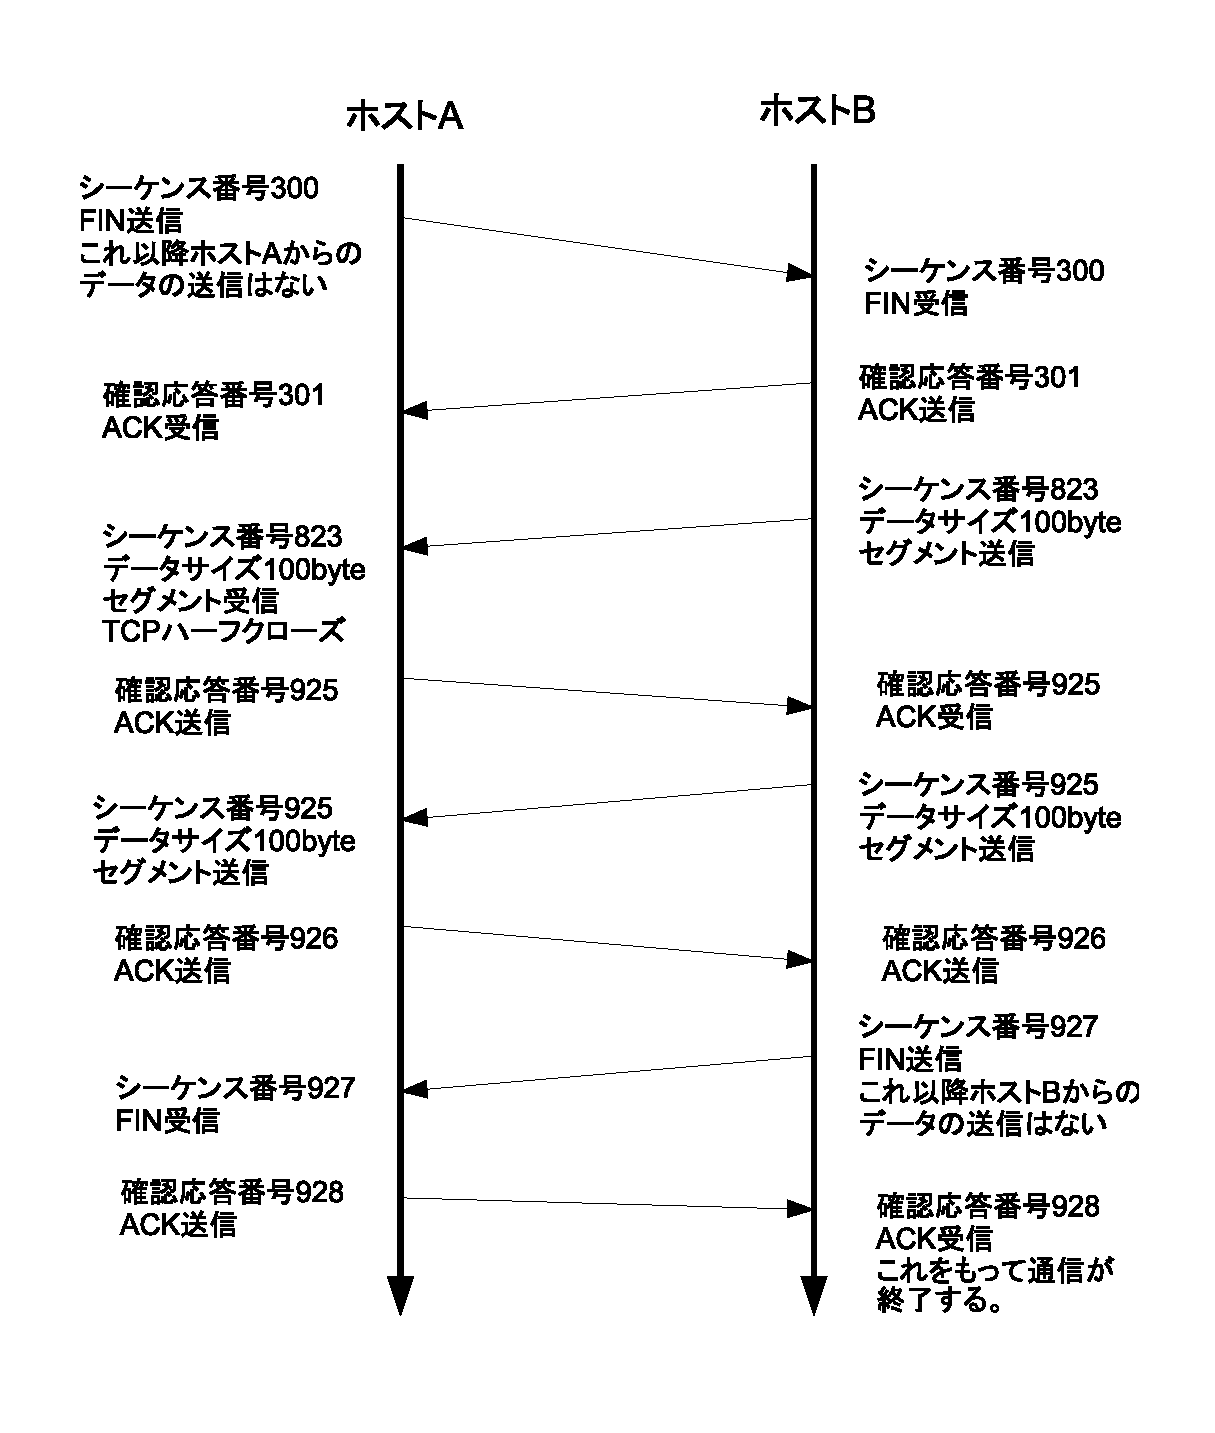
\includegraphics[width=6cm, clip]{draw/tcp06n.eps}
	\caption{TCPハーフクローズ}
	\label{fig:tcp06}
\end{wrapfigure}


ホストBは、データの送信が完了したら、ホストAにFINを送信する。この時点で、ホストBから送信されるデータがもうないことが、ホストAに通知された。それに対してホストAがACKを返したら、ホストA、ホストBとも、相手から来るデータはもうない、ということを知ったことになる。それ以降の通信は行われず、それをもってコネクションが切断されたということになる。


では、なぜコネクションの切断に関しては、ハーフクローズという概念が存在するのだろうか?FINに対してACKを返した時点で、コネクションが切断されてもいいのではないか、そのような疑問をもったのではないだろうか。

TCPでは、通信を行っているプロセスはそれぞれ独立して存在し、お互いを関知せずに動作している。そのため、送信が終わった、という通知も独立して行うべきであるという思想がその根底に存在する。そのために、双方が通信の終了を宣言し、双方が確認応答しないと、コネクションは切断されない。

また、リモートシェル系のアプリケーションは、ハーフクローズを積極的に使用する。rshなどのリモートシェルでは、クライアント側がシェルコマンドを送信した時点でハー風クローズし、サーバ側は実行結果をハーフクローズ状態でクライアントに返し、その後コネクションを切断する。

\subsection{遅延ACKとピギーバック(piggy back)}
\begin{wrapfigure}[22]{r}{7cm}
	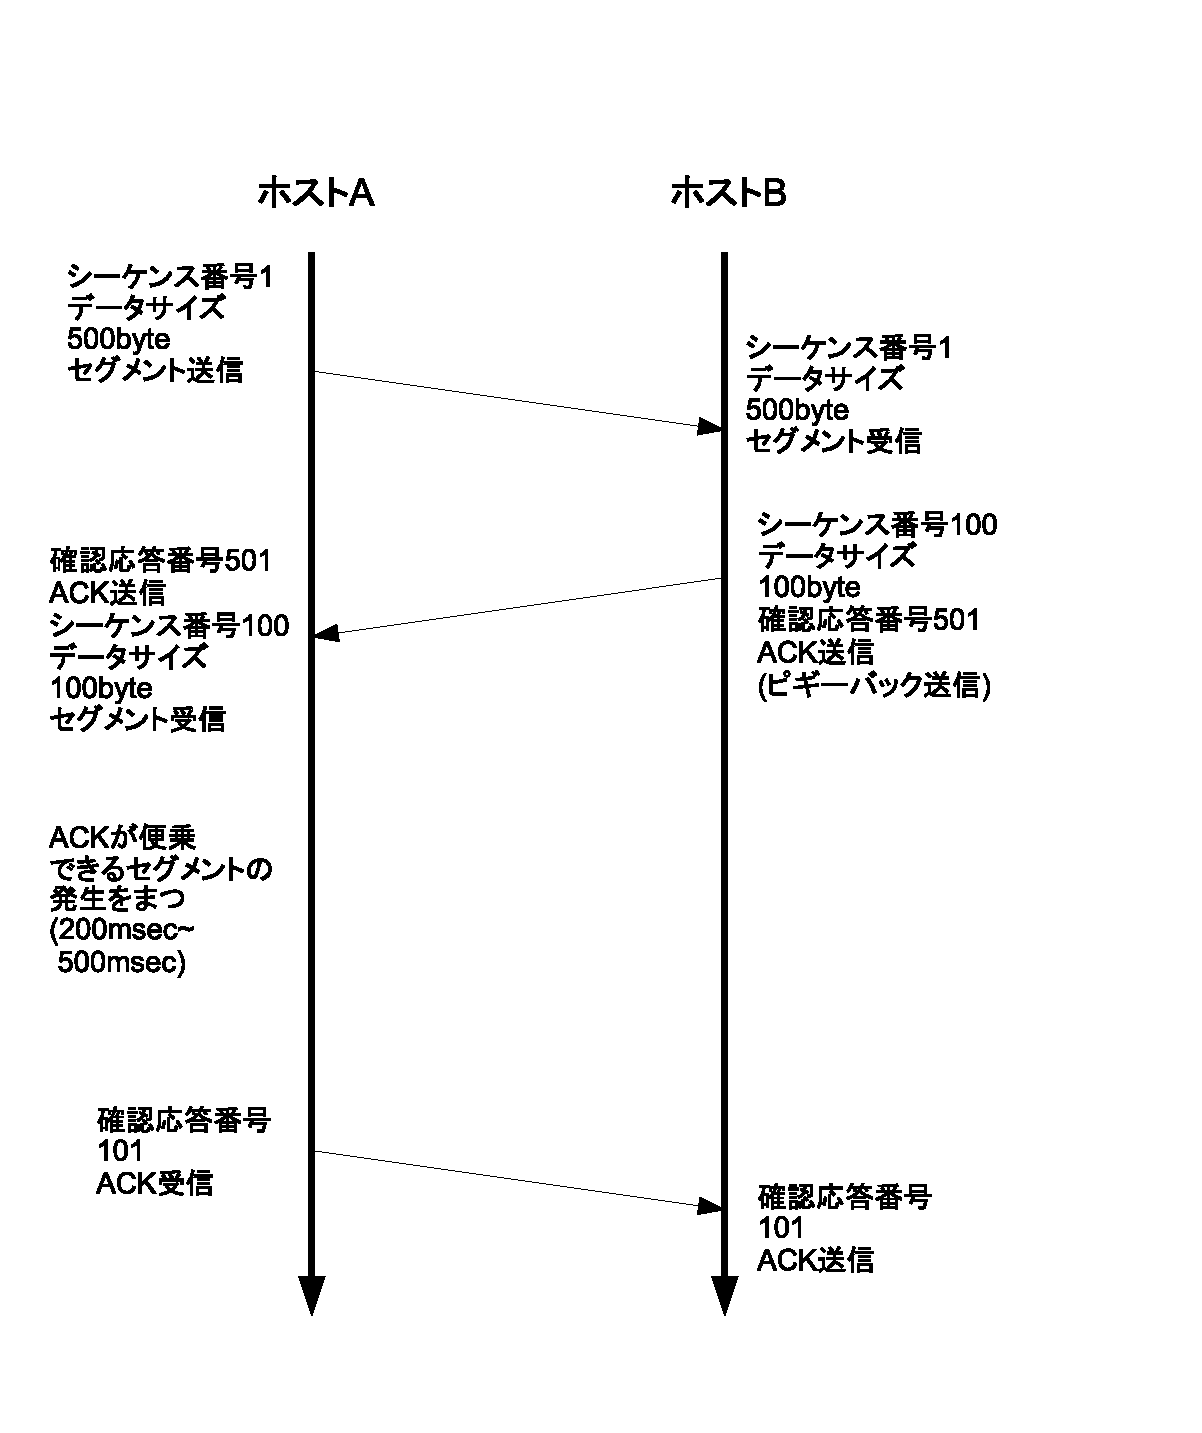
\includegraphics[width=7cm, clip]{draw/tcp03n.eps}
	\caption{遅延ACKとピギーバック}
	\label{fig:tcp03}
\end{wrapfigure}

TCPでは、セグメントを受信すると、それに対してACKを返す。このACKとはどのようなものかを、改めて考えてみよう。

ACKは、TCPのヘッダにあるACKフラグを有効にし、ヘッダ内の確認応答番号のフィールドに、次に送ってほしいセグメントの番号を入れたものである。つまり、ACKも、TCPのセグメントとして送信される。

ここで、ACKをひとつ送信するコストを考えてみよう。ACKを一つ送信するのに、TCPヘッダのみの、20オクテットの大きさを持つセグメントを送信する必要がある。当然、このセグメントをインターネットプロトコルで送信するために、IPヘッダの20オクテットが追加される。つまり、ACKひとつを伝送するために、40バイトのデータをネットワークアクセス層に流さなければならない。\footnote{実際には、ネットワークアクセス層のヘッダやトレイラの分も追加される。}

これは、回線速度が遅い時代には、それなりに重い負荷であった。たかがACK一つ送信するのに、320bitものデータを流さなければならないのだ。また、ACKひとつで一つのIPデータグラムとなるので、経路にあるルータの負荷を増すし、まわりまわってACKが途中で捨てられてしまう可能性もないとは言えない。そのため、単独でACKだけを送信する状況が発生しないようにしたかった。


そこで、ACKを送信する必要が生じた場合、ACKを送信する側に、ACKを送信する先に送る、ACK以外のセグメントが発生しないか、一定時間待つ。そのようなセグメントが生じたら、ヘッダにACKの情報を便乗させる。これは、ACKの情報である確認応答番号が、TCPヘッダの中で独立したフィールドをもってしていることで可能となる。

このように、送信されるセグメントのヘッダにACKの情報も一緒に載せて送ることを、ピギーバック(piggy back)という。日本語にすると親亀子亀のスタックや、便乗という言葉をイメージすればいいだろう。

通常、ACKを送信する際は、ピギーバックできるセグメントがないか200msec待つ\footnote{規格では500msec待ってかまわない。}そして、待ち時間を過ぎてもピギーバックできるセグメントがなければ、ACKはACKだけで送信される。この、便乗できるセグメントがないまま待ち時間いっぱい待って、その後で送信されるACKを、遅延ACKと呼ぶ。

ACKは通常、ピギーバックもしくは遅延ACKとして送信される。だが、セグメントを受信した後にすぐACKを送信しなければならない場合があるため、 OSの実装毎に、遅延ACKを抑止する方法が用意されている。


\section{相手が受信できるだけデータを送る}

TCPでは、確実な通信を行うために、相手が受信できるだけのデータを送信する機能がある。

TCPでは、セグメント毎にACkを返すことになっている。だが、ACKの到着を待って次のデータを送信していたら、セグメント一つ送信するごとに、セグメントとACKで一往復となり、時間がかかる。送信すべきデータがあらかじめ存在し、その大きさがそれがMSSより大きい、つまり、複数のセグメントを送信しなければならないことが分かっている場合、それは時間がかかってしまう。

そのような場合、ACKを待たずにある程度のデータをまとめて送信してしまい、後でそれらのACKをまとめて受信すればいいのではないだろうか。TCPでは、MSSより大きいデータを送信する場合は、複数のセグメントを、ACKを待たずに送信することができる。だが、ここで一つ問題がある。ACKを待たずに、どのくらいの量のデータを送信していいのだろうか。

\subsection{受信バッファと送信量制御}

トランスポート層が受信したが、まだアプリケーション層に引き渡されていないデータを貯留する小さなメモリを、受信バッファ、もしくは単にバッファと呼ぶ。送信側が送出したデータの総量が大きすぎれば、バッファに入りきらないデータが捨てられる。それは、確実な通信の妨げになるだろう。この受信バッファとは、TCPが受信に使用する領域である。

そこで、TCPでは、受信側に、その時点で受信可能なデータの総量を自己申告してもらう、という方法をとっている。TCPヘッダには、その大きさを自己申告するためのフィールドが予約されている。そのフィールドを、ウインドウ・サイズという。

今回も、TCPの通信で、送信する側をホストA、受信する側をホストBとして説明しよう。ホストBは、ACKを返すときなど、ホストAに何らかのセグメントを送信する毎に、受信したデータを一時的に置いておくバッファの大きさがどれだけ残っているかを、TCPヘッダのウインドウ・サイズに入れて送信する。バッファの大きさを伝えることを、ウインドウ・サイズ広告という。ウインドウ・サイズは、それが広告された時点でのバッファの残りである。では、ウインドウ・サイズ分いっぱいのデータを送信しても大丈夫ということだろうか?

\begin{wrapfigure}[27]{r}{7cm}
	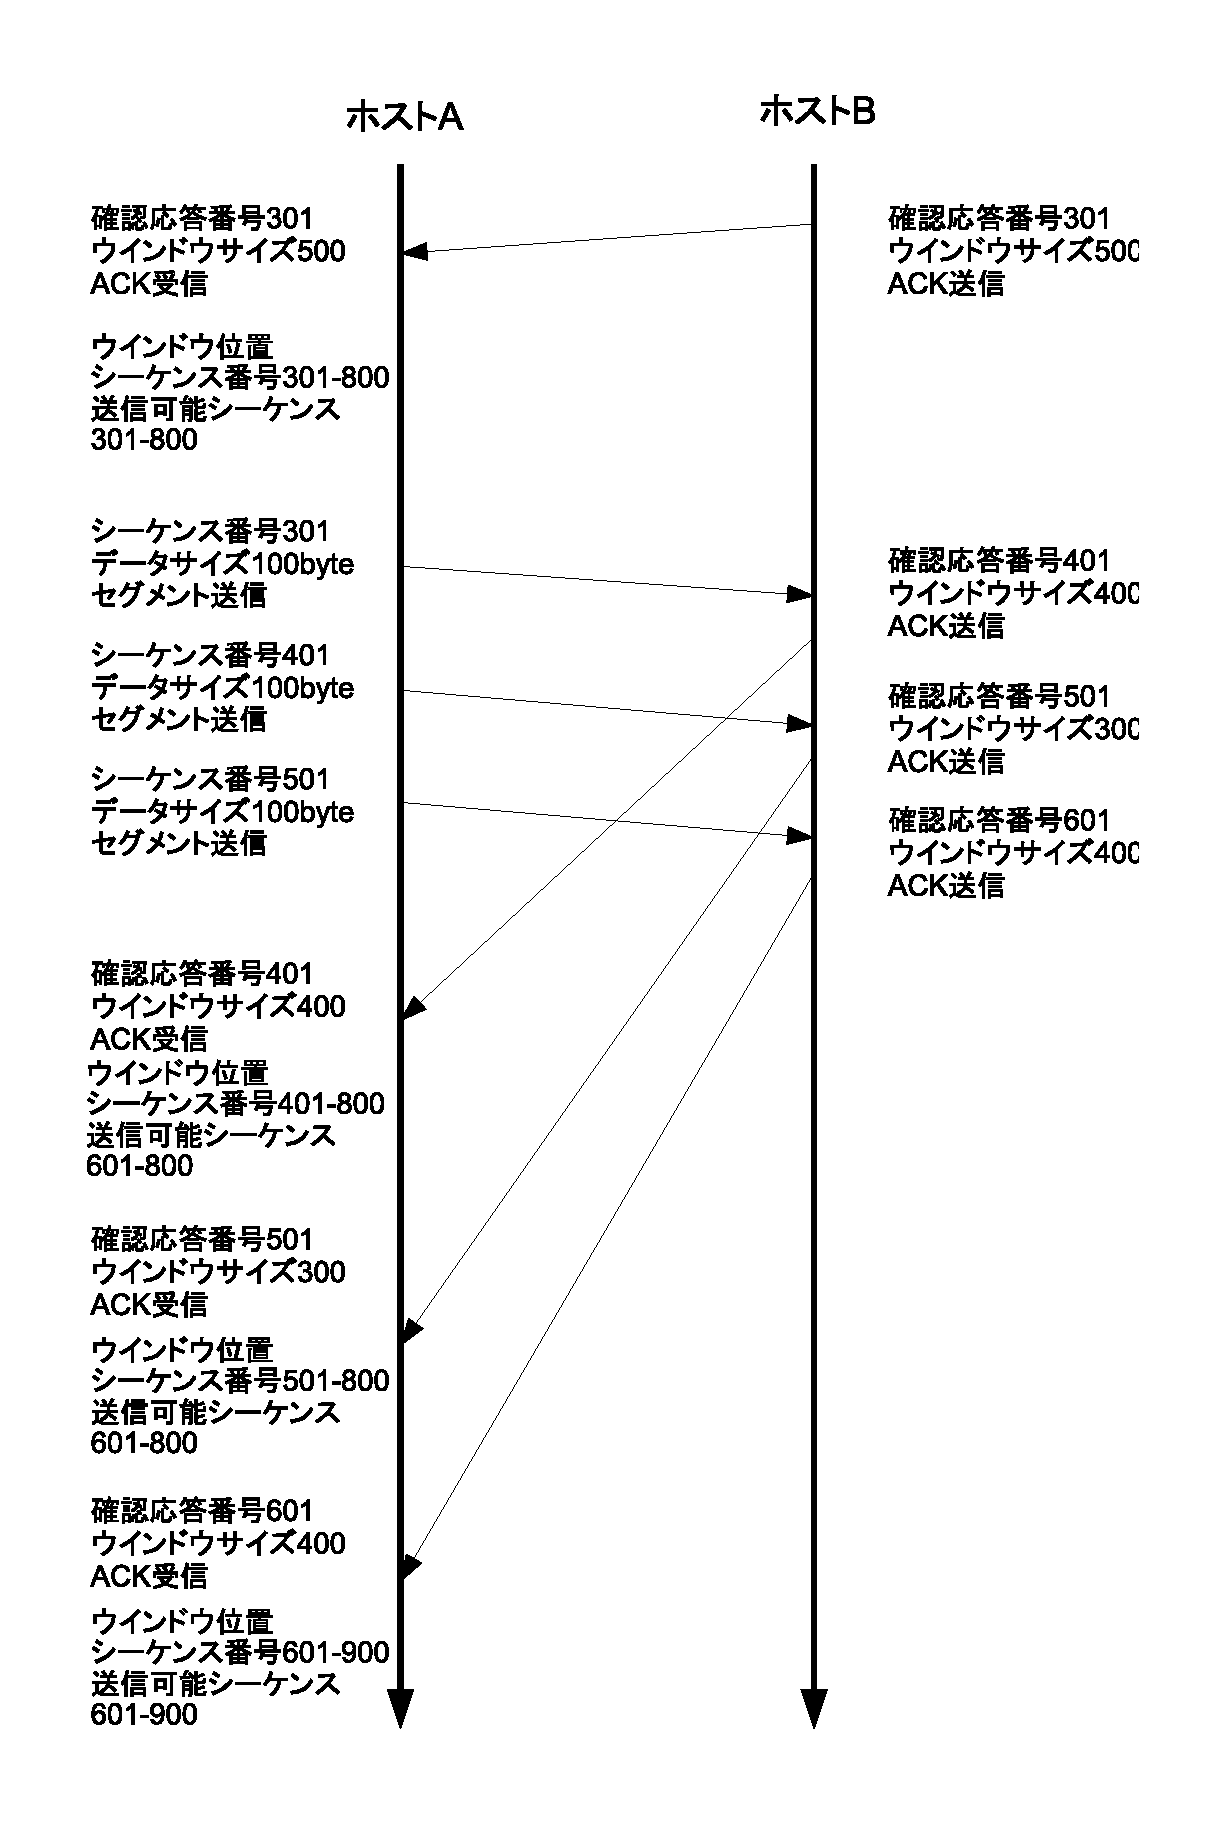
\includegraphics[width=7cm, clip]{draw/tcp07n.eps}
	\caption{バルク送信とウインドウサイズ広告}
	\label{fig:tcp07}
\end{wrapfigure}

ホストAが、ホストBからのウインドウサイズ広告のついたACKを受信した時点で、ホストAが送出したセグメントのうち、対応するACKが戻ってきていないものが、いくつかあったとする。そのセグメントは、これから受信バッファに取り込まれるだろうから、受信バッファを消費することになる。そこで、ウインドウ・サイズ広告から、送出したがACKが戻ってきていないセグメントの、データの総量を引く。そして残ったのが、これからACKを待たずに送信可能なデータの量となる。

では、受信側が自己申告する受信バッファの大きさを、ウインドウ・サイズというのはなぜだろうか。それは、ここまでの説明を、図にしてみることで理解することができるだろう。

まず、送信側が送信するストリームを、一直線に並べる。ここでは、説明をし易くするために、ISN=0,MSS=1として話を進めよう。送信したいデータと、シーケンス番号を一直線に並べると、以下の図のようになる。

\begin{figure}[h!] \caption{ウインドウサイズ広告(1)} \label{windowsize1}
\begin{center}
{\scriptsize
\begin{verbatim}
Stream     H  E  L  L  O sp  W  O  R  L  D sp  T  H  I  S sp  I  S sp  F  I  N  E sp  D  A  Y lf cr              
         +--+--+--+--+--+--+--+--+--+--+--+--+--+--+--+--+--+--+--+--+--+--+--+--+--+--+--+--+--+--+......
Seq #      1  2  3  4  5  6  7  8  9 10 11 12 13 14 15 16 17 18 19 20 21 22 23 24 25 26 27 28 29 30  
\end{verbatim}
}
\end{center}
\end{figure}

ここで、確認応答番号1のACKと共に、ウインドウ・サイズ5が戻ってきたとしよう。この場で一度に送信できるのは、シーケンス番号1から数えて5セグメント分である。これを図示すると、以下のようになる。

\begin{figure}[h!] \caption{ウインドウサイズ広告(2)} \label{windowsize2}
\begin{center}
{\scriptsize
\begin{verbatim}
_________|<WindowSize >|      
Stream     H  E  L  L  O sp  W  O  R  L  D sp  T  H  I  S sp  I  S sp  F  I  N  E sp  D  A  Y lf cr              
         +--+--+--+--+--+--+--+--+--+--+--+--+--+--+--+--+--+--+--+--+--+--+--+--+--+--+--+--+--+--+......
Seq #      1  2  3  4  5  6  7  8  9 10 11 12 13 14 15 16 17 18 19 20 21 22 23 24 25 26 27 28 29 30  
\end{verbatim}
}
\end{center}
\end{figure}

この図でわかるように、ウインドウ・サイズとは、送信側が送出するストリームの上に開いた、「この部分を送出する」という窓(ウインドウ)である。

では、この状態でホストAが3セグメント分のデータを送出し、ホストBからACK 3 ウインドウサイズ3が帰ってきたとしよう。

\begin{figure}[h!] \caption{ウインドウサイズ広告(3)} \label{windowsize3}
\begin{center}
{\scriptsize
\begin{verbatim}
_______________Window Size
_______________|<----->|      
Stream     H  E  L  L  O sp  W  O  R  L  D sp  T  H  I  S sp  I  S sp  F  I  N  E sp  D  A  Y lf cr              
         +--+--+--+--+--+--+--+--+--+--+--+--+--+--+--+--+--+--+--+--+--+--+--+--+--+--+--+--+--+--+......
Seq #      1  2  3  4  5  6  7  8  9 10 11 12 13 14 15 16 17 18 19 20 21 22 23 24 25 26 27 28 29 30
ACK            |<-ACK 3  
Sent           ->|
\end{verbatim}
}
\end{center}
\end{figure}

窓の左端は、受信したACKの確認応答番号で、一番大きいものに一致するシーケンス番号を持つセグメントとなる。送信したセグメントのうち、シーケンス番号が一番大きいのは3だが、戻ってきたACKの確認応答番号で一番大きいものは3である。そのため、送出したセグメントのうちシーケンス番号3は、まだ受信側のバッファに入っていないことが分かる。この状況で送出可能なデータの量は、ウインドウ・サイズの3から、送出したがまだバッファに入っていないデータの大きさ1をひいて、2となる。つまり、シーケンス番号4とシーケンス番号5の、合計二つのセグメントを送出できることが分かる。

シーケンス番号4と5のセグメントが送信された状態で、今度はACK4 ウインドウサイズ4が戻ってきたとしよう。つまり、シーケンス番号1と2に相当するデータが上位のアプリケーションに渡され、その分のバッファが空いた状態である。この状態の図を書くと、以下のようになる。

\begin{figure}[h!] \caption{ウインドウサイズ広告(4)} \label{windowsize4}
\begin{center}
{\scriptsize
\begin{verbatim}
___________________Window Size
__________________|<-------->|      
Stream     H  E  L  L  O sp  W  O  R  L  D sp  T  H  I  S sp  I  S sp  F  I  N  E sp  D  A  Y lf cr              
         +--+--+--+--+--+--+--+--+--+--+--+--+--+--+--+--+--+--+--+--+--+--+--+--+--+--+--+--+--+--+......
Seq #      1  2  3  4  5  6  7  8  9 10 11 12 13 14 15 16 17 18 19 20 21 22 23 24 25 26 27 28 29 30
ACK               |<-ACK 4  
Sent                 ->|
\end{verbatim}
}
\end{center}
\end{figure}

このように、ウインドウの左端はACKによって右方向に移動する。一方、ウインドウの右端は、バッファが空くことで、右側に移動する。ウインドウサイズが小さくなるのは、ウインドウの右端が右に動く量よりも、左端が右に動く量の方が多い場合である。また、ウインドウサイズが大きくなるのは、ウインドウの左端が右に動く量より、右端が右に動く量の方が大きい場合である。これらの動作が、引き戸の窓を左右に動かすように見える。そのため、この方法によるデータ総出量の調整を、スライディングウインドウという。

スライディングウインドウでは、窓の右端、左端とも、右に動くことはあっても左に動くことはない。また、窓の左端が、その窓の右端に追いついた状態を、ゼロウインドウと呼ぶ。ゼロウインドウのときは、いわば窓が閉じた状態であり、受信バッファに空きがないことを意味する。そのため、ゼロウインドウのときはデータを送信しない。

スライディングウインドウで注意すべきなのは、これは送信側が、受信側のウインドウ・サイズ広告と、ACKの到着状況と送出済セグメントの関係から割り出した、送信側の主観によるものであるということである。TCPにおいて、そのセグメントの送出量を制御する第三者はいない。そのため、ウインドウサイズに合わせての送信は、、送信側が自主的に行う必要がある。

\subsection{送り直しとデータの送信量の制御}

TCPでは、受信側が受信できなかったデータの再送と、送信量の制御はほぼ一体となっている。TCPの重要な機能として、最後にこれらを説明しよう。まず、ここで言う送信量とは、先度説明したスライディングウインドウではなく、途中の経路の状況に応じて調整する送信量である。

\subsection{再送信が必要な状況}

TCPで、データ(セグメント)の再送信が必要になるのはどのような状況であろうか。まずそれを見ていこう。

まず、TCPでは、セグメントが途中で失われた、もしくはセグメントが破損していたということを送信側が知るには、どのようにするのかを振り返ってみよう。TCPでは送信側は、時間内にACKが返らないということを目安に知ることができる。このとき、全てのセグメント不着の事例において、セグメントの破損は1パーセント以下の確立でしか発生しないとされる。それは、IPヘッダが破損せず、IPヘッダのチェックサムに矛盾が生じず、TCPのセグメントだけ破損するという事例はほとんど生じないためである。つまり、セグメントの不着や破損は、下位のサー^ビスが原因となって発生することのほうが、圧倒的に多い。

そのため、ACKが時間内に戻らないタイムアウトは、経路の途中で、TCPから見た下位のサービスの能力以上の通信があったために、到着していないと考えることができる。その状況で確実な通信を行うためには、相手に届かなかったと思われるセグメントを再送信すると共に、ACKを待たずに送信していたデータの量を減らす必要がある。そのため、TCPではセグメントの再送信と送信量の制御が一体になっている

\subsubsection{ACKで状況を伝え、確認する}

TCPでは、送信側に、受信側からのACKが返ったことで、それに対応するセグメントは受信されたと判断する。では、ACKを用いて、セグメントが受信されなかったことを知るにはどうすればいいだろうか。これをケース別に考えてみよう。

\subsubsection{ACKが時間内に届かなかった}

あるセグメントに対応するACKが時間内に到着しなかった場合、TCPでは、そのセグメントを再度送信しなおす。このとき、セグメントを再送信する毎に、タイムアウトの待ち時間を増加させる。

\subsubsection{重複ACKが届いた}



以下のような状況で、重複ACKという、同じ確認応答番号を持つACK画幅数回到着する現象が発生する。

\begin{wrapfigure}[27]{r}{7cm}
	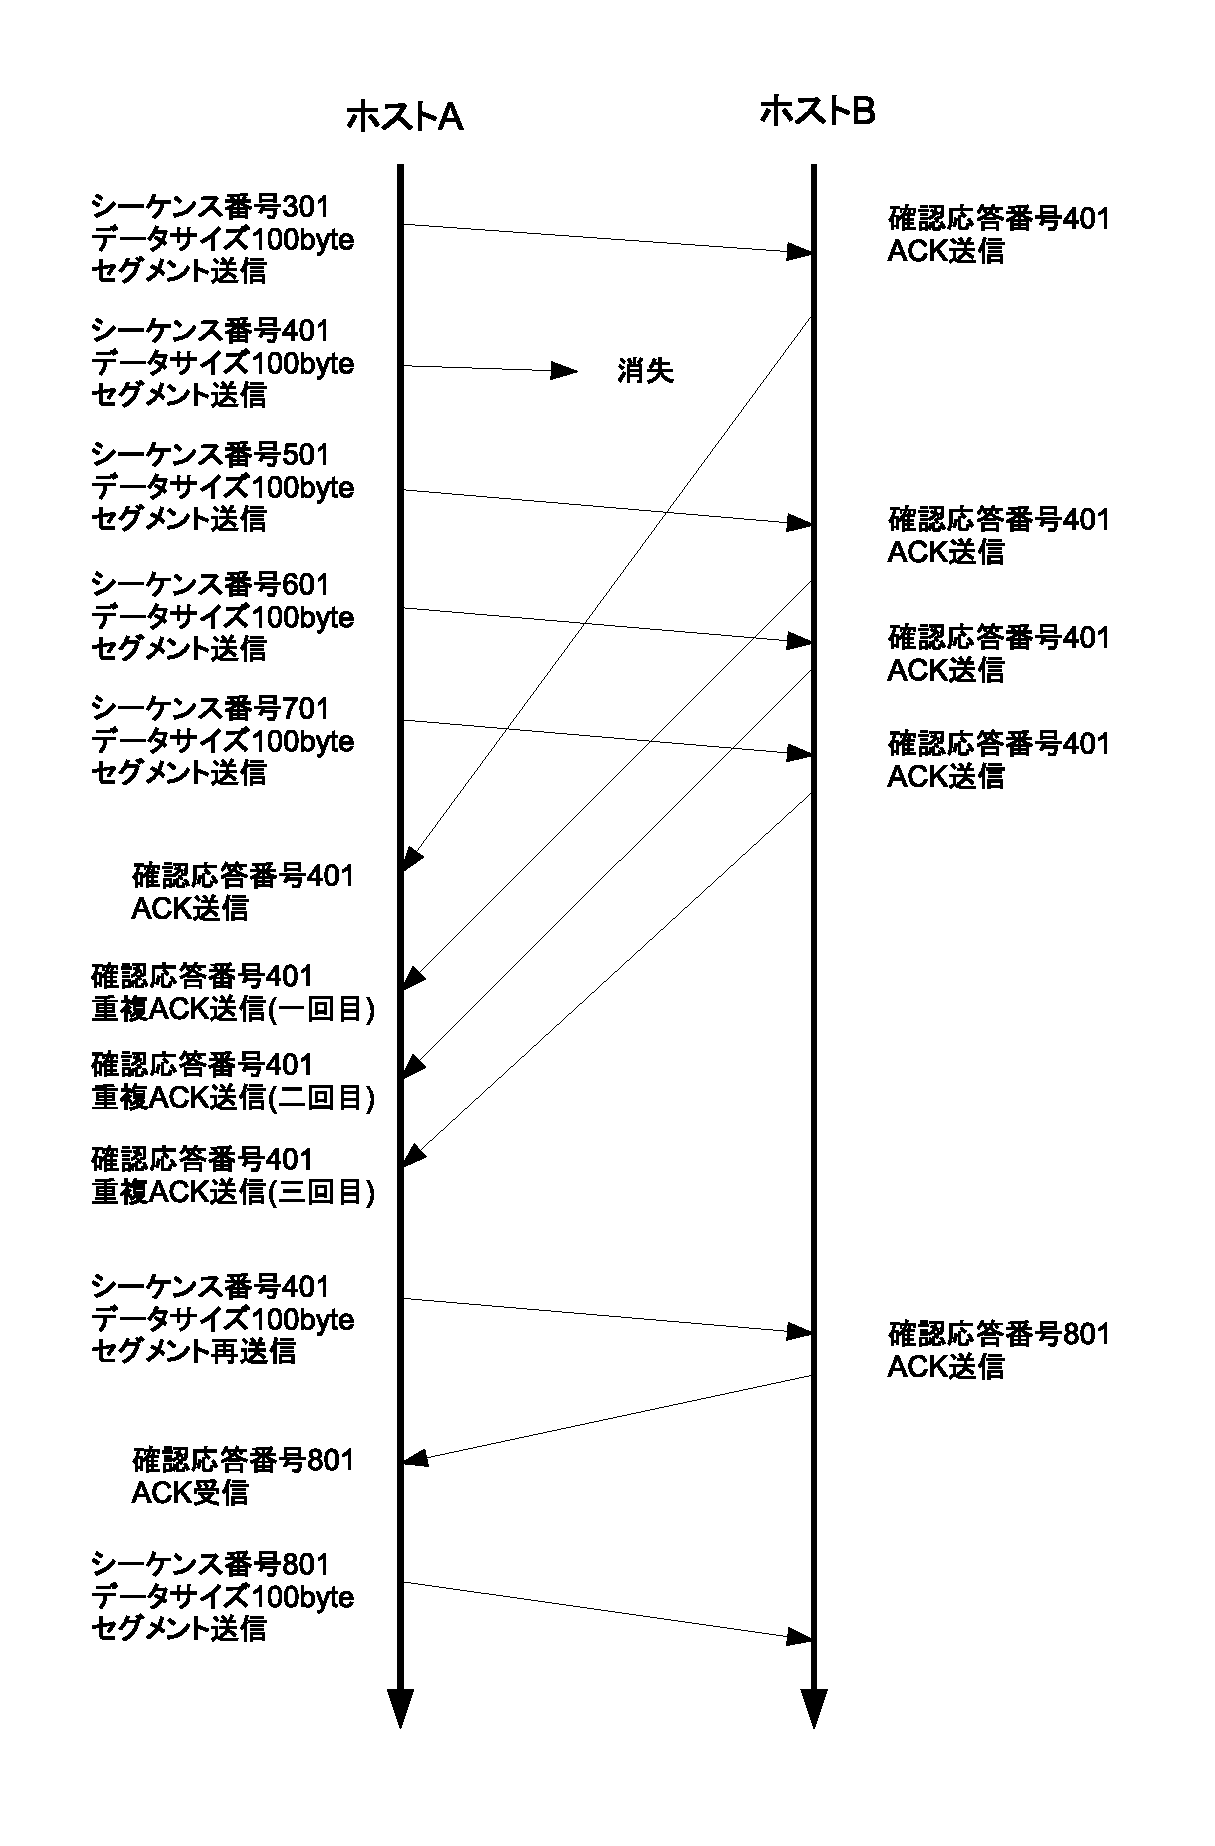
\includegraphics[width=7cm, clip]{draw/tcp08n.eps}
	\caption{重複ACK}
	\label{fig:tcp08}
\end{wrapfigure}

TCPの通信において起こりうるのは、スライディングウインドウに従って、まとめて送出したセグメントのうち一部が届かない、ということである。この場合、シーケンス番号順に到着せず、順番が前後した場合と、セグメントが届かなかった場合とがある。

前者の場合、受信側は、到着したセグメントのもつシーケンス番号から、届かなかったセグメントが存在することを知ることができる。シーケンス番号の順番通りにセグメントが届かなかった場合、受信側は、届かなかったシーケンス番号を持つセグメントが到着するまで、他のセグメントが到着する毎に送出するACKの、確認応答番号を、届かなかったとおもわれるセグメントのシーケンス番号に対応するものとする。





この確認応答番号のACKは、届かなかったシーケンス番号のセグメントが到着するまで送出される。この、同じ確認応答番号をもって複数回送出されるACKを、重複ACKという。

重複ACKを受信した送信側は、その数を数える。重複数が1もしくは2(同じ確認応答番号のACKがふたつもしくは三つの場合)で、それ以降確認応答番号が、送出したセグメントに応じて増加していった場合は、シーケンス番号通りではないが、セグメントは到着したことが判る。

重複ACKの重複数が3を越えたら、つまり同じ確認応答番号のACKが4個を越えたら、それは途中でセグメントが失われたと判断する。送信側は、重複ACKの確認応答番号に対応するシーケンス番号を持つセグメントを、再送信する。

\subsection{輻輳の回避}

TCPにおける通信の送出量は、スライディングウインドウで通知される、受信側の現時点での受信能力という上限が存在する。だが、それに達していなくても、到着しなかったり順番が入れ替わったりするセグメントが発生する。それはすなわち、通信の経路がその伝送能力を超えた状態にあるのではないか、そう考えるべきであろう。通信の経路をその処理能力以上のデータが通ろうとしていて、結果、データグラムが捨てられる状況を、通信の言葉で輻輳(ふくそう)という。

ここでは、その輻輳の回避について、簡単に説明をしたい。

TCPでデータを送信する際は、最初から、受信側が通知したウインドウサイズ一杯のデータを送信するわけではない。最初は1セグメントから送信を開始し、ACKが戻る毎に、 ACKを待たずに送信するセグメントの数を増やしていく。そのように、ACKを待たず送出するセグメントの数を増やしていくと、ACKが時間内に返らなかったり重複ACKが返ったりする現象が起こる。この場合、途中の経路で輻輳が起こっている可能性がある。

ACKが時間内に返らない場合は、途中の回線がかなり輻輳していると推測できる。そのため、ACKを待たずに送信するセグメントの数を1に戻す。

重複ACKの場合は、輻輳が発生した瞬間があったが、その前後で通信は行われていた状況である。そのため、ACKを待たずに送信するセグメントの量をそれまでの半分にして、そこからまた、ACKを待たずに送出するセグメントの数を増やしていく。

この輻輳回避を行うことで、ACKを待たずに送信されるセグメントの数は、その時点の最適値の周りで振動収束する。



\subsection{タイムアウト}

\begin{wrapfigure}[20]{r}{7cm}
	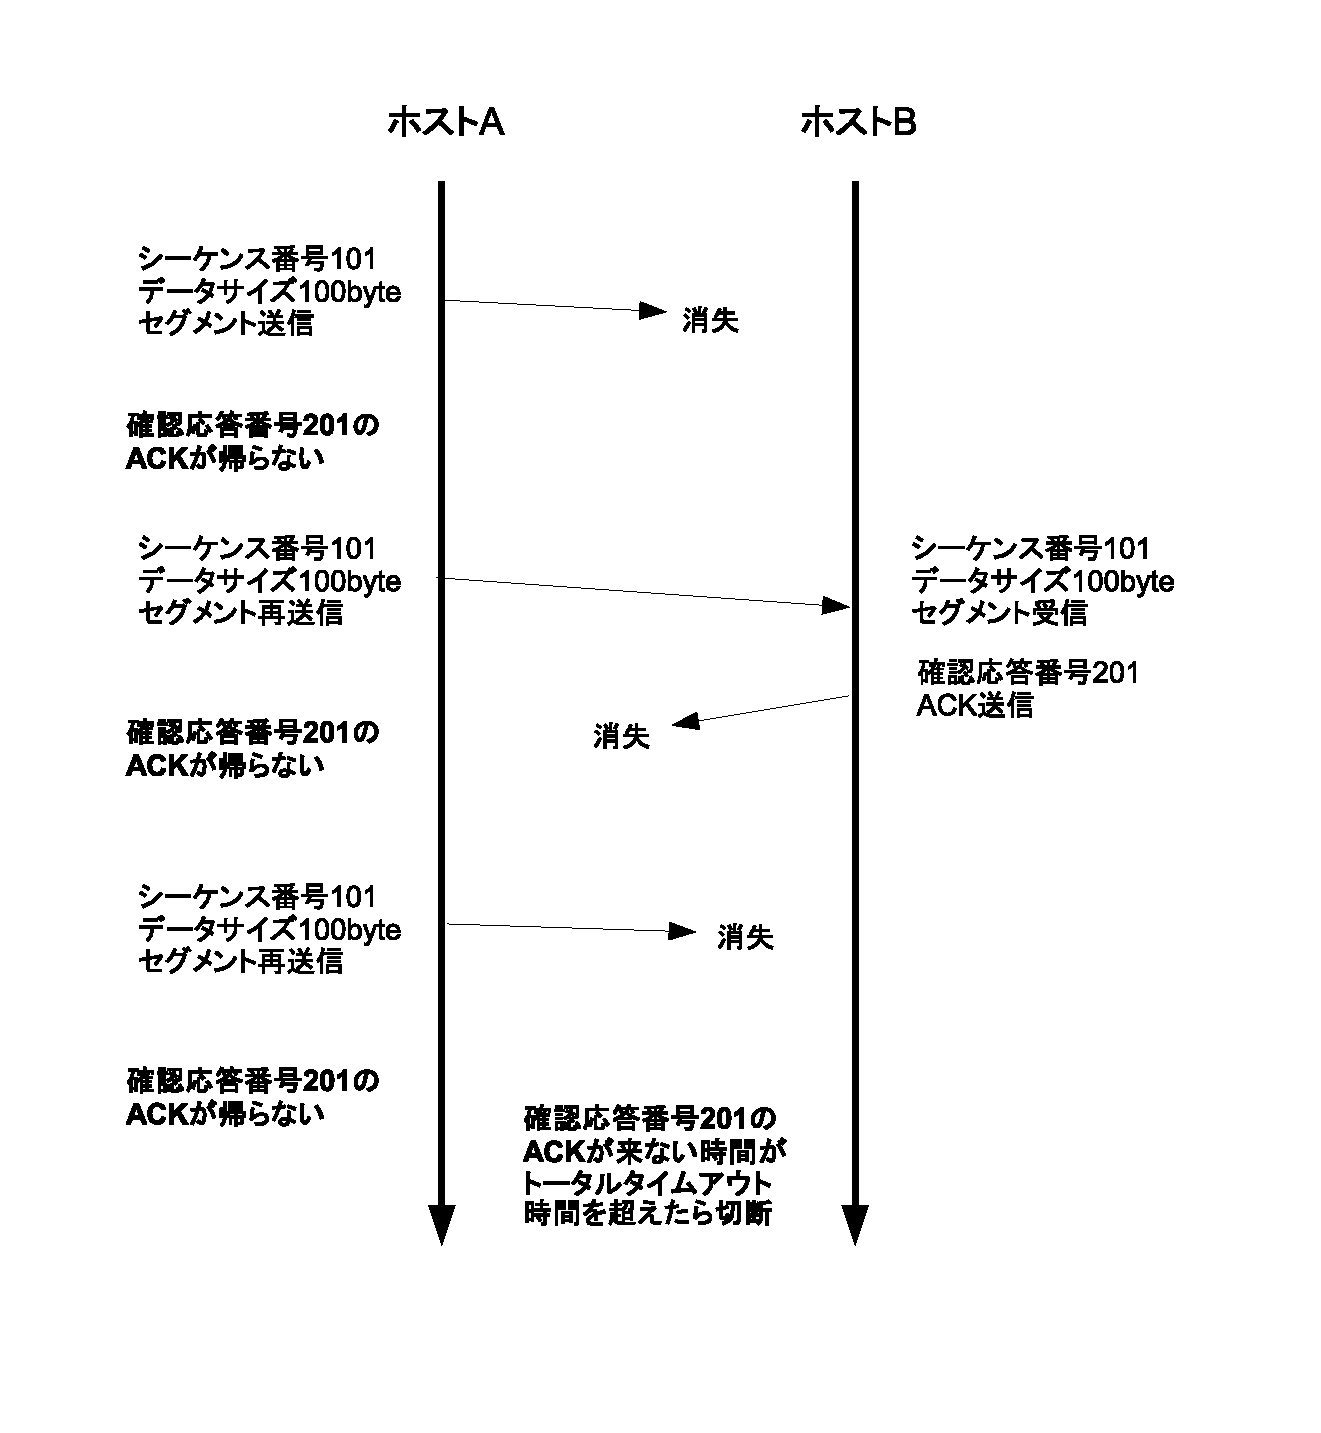
\includegraphics[width=7cm, clip]{draw/tcp09n.eps}
	\caption{タイムアウト}
	\label{fig:tcp09}
\end{wrapfigure}

最後に、TCPにおけるタイムアウトについて説明しよう。ここまで何となくタイムアウトという言葉を用いてきたが、具体的に何秒待てばタイムアウトになるのか、という説明はしなかった。それは、TCPにおけるタイムアウトは、あるセグメントを送出して、それに対応したACKが戻ってくるまでの時間を評価して、決定するためである。



あるセグメント送信後、それが到達しなかったとみなして、再度おなじシーケンス番号をもつセグメントを送出するまでの時間を、再送時間(RTO Resend Time Out)という。実測値からRTOを決定するには、古典的な方法とJacobsonの提案によるものの二種類がある。現在では、実測値のばらつきを考慮してあり、整数演算かつ係数の乗除算がシフト演算で行えるJacobsonの方法が用いられることが多い。古典的な方法は、実数演算を行う必要があるため、Jacobsonの方法より演算のりソースを必要とする。

あるセグメントのタイムアウト時間は、再送を行う毎に、指数関数的に増加していく。タイムアウトは、コネクション毎でなく、セグメント毎に測定される。このタイムアウト時間の合計が、トータルタイムアウト時間、という時間に達したら、TCPは通信が不可能であると判断し、コネクションを切断する。トータルタイムアウト時間は、約9分に設定され、多くのTCPの実装で変更することはできない。そのため、アプリケーションの実装で、もっと短い時間で切断するよう実装することが多い。

\section{TCPヘッダ}

\begin{figure}[htbp]
	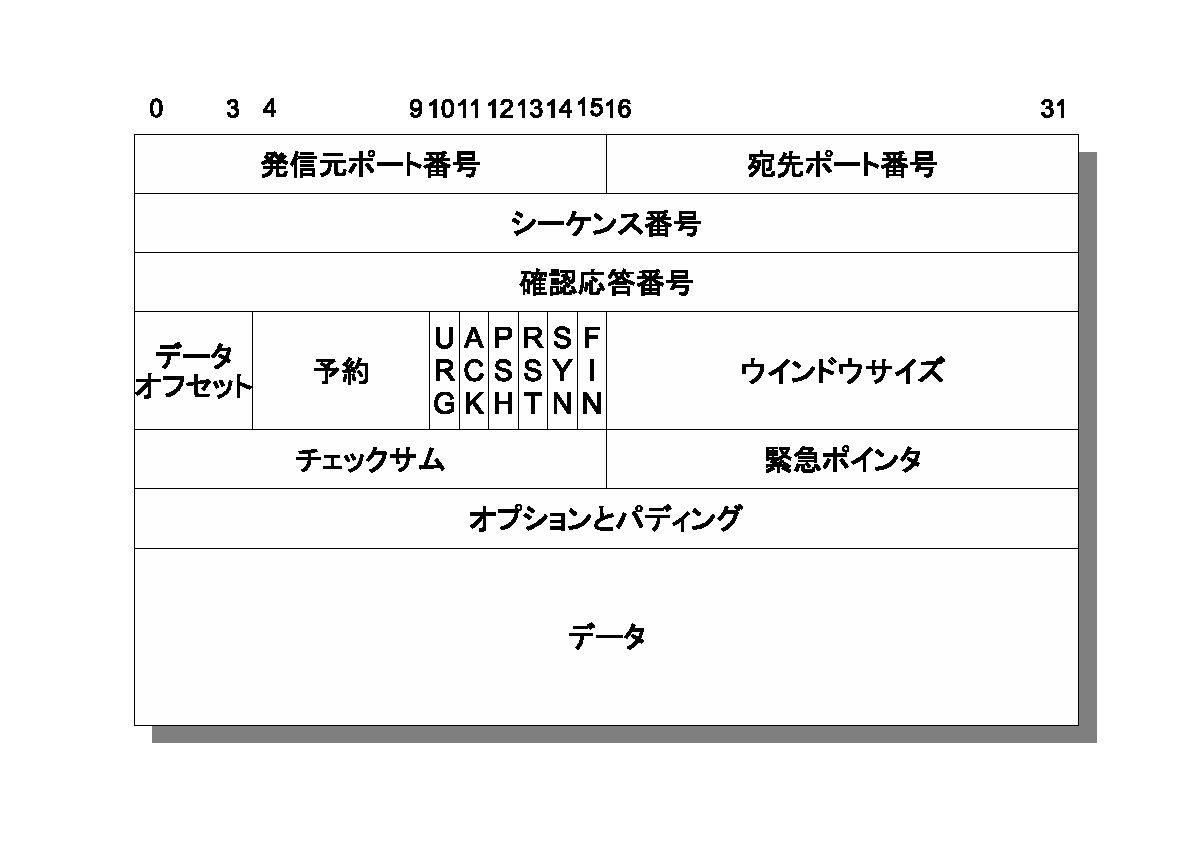
\includegraphics[width=12cm,clip]{draw/tcpheader.eps}
	\caption{TCPヘッダの構造}
	\label{fig:tcpheader}
\end{figure}

TCPのヘッダの構造は、図\ref{fig:tcpheader}のようになる。ここまでの説明で登場しなかったデータを収めるフィールドについて、説明をしていく。

\subsection{オプションフィールド}
TCPヘッダには、任意長のオプションフィールドがある。このオプションフィールドは、TCPの機能拡張などに用いられている。

フォーマットは、先頭から、kind、size、オプションのデータとなる。サイズフィールドは、先頭2byte(kind,size)を含んだ大きさとなる。オプションは定義されている限り、いくつ連続させてもよい。

オプションフィールドは将来拡張に用いられる。また、受信側は、未実装のオプションを受信したときはこれを無視してよい。そのため、未実装のオプションの「読み飛ばし」を可能にするため、sizeフィールドが存在する。

オプションフィールドの最後はkind=0を記入する。また、kind=1のNOPは、オプションフィールドをワード境界に保つためののパディングに用いる。この二種類のkindは、サイズフィールドを省略する。

オプションフィールドは、NOPを入れるか、末尾に0を連続させ、32bit境界に揃える。

\begin{figure}[htbp]
	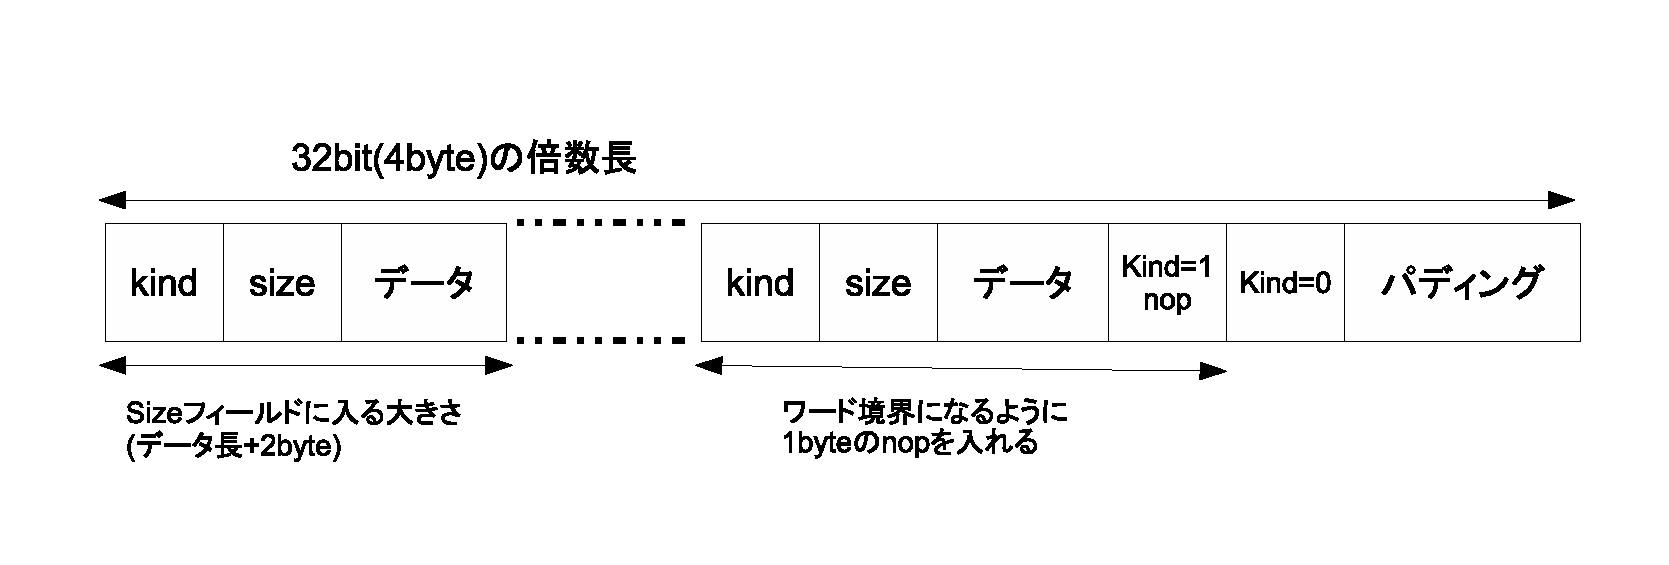
\includegraphics[width=12cm,clip]{draw/tcpopt.eps}
	\caption{TCPオプションフィールド}
	\label{fig:tcpopt}
\end{figure}


\subsection{オプションフィールドの例 kind=2 MSS}
オプションフィールドの使用例として、kind=2の最大セグメント長(Maximum Segment Size MSS)について説明しよう。

TCPのセグメント長は、どのくらいの大きさにすればよいのだろうか。TCPにサービスを提供するインターネットプロトコル層のデータグラムは、最大64kByteである。だが、インターネットプロトコルが利用するネットワークアクセス層の最大転送単位(Maxuimum Transfer Unit MTU)はそれよりずっと小さい。

インターネットプロトコル層で、ネットワークアクセス層にMTUの大きさににあわせたセグメンテーションが行われる。それを考えると、MTUから各層のヘッダの大きさを引いたものより小さくすればよいのではないかという見当がつくだろう。\footnote{最適なMSSを動的に算出するのがパスMTUディスカバリという方法である。本書では詳細には立ち入らないので、これもまた興味があれば各自調べてみていただきたい。}

では、何らかの形で決定したMSSも、自分が通信相手にに向けて送信する場合のみでなく、相手から自分に送信してもらうときにもそのサイズにしてもら割らないと意味がない。そこで、通信相手にMSSを通知するのに用いるのが、kind=2である。

\subsection{ACKフラグ}
TCPでACKを送出するときは、TCPヘッダのACKフラグを1にする。

ここまで説明したように、ACKフラグは、通信相手に確認応答番号までのデータを受信したことを伝える。ACKは、3wayハンドシェイクのときや、遅延ACKを使用しない場合、タイムアウトまでにピギーバックできるTCPセグメントが発生しなかった場合など、ACKフラグが有効になったTCPヘッダのみで送出されることがある。

だが、それ以外の場合は、他のデータ送信時のヘッダに、確認応答番号とACKフラグの情報を乗せる、ピギーパックで送出されることが多い。

\subsection{SYNフラグ}
TCPのコネクションの開始を要求するときは、SYNフラグを1にしたTCPヘッダを送出する。繰り返すが、SYNフラグが有効になったTCPヘッダを送出した次点では、コネクションは成立していない。コネクション成立の応答のために存在するフラグである。

通信相手からSYNでコネクションの要求をされた側は、SYNフラグを有効にしたヘッダに、ACKをピギーバックして送出する。つまり、SYNフラグとACKフラグが有効になったTCPヘッダのみを送出する。

\subsection{FINフラグ}
FINフラグは、コネクションの終了を通信相手に通知するのに用いる。FINフラグの有効なTCPヘッダを受信割いたら、今後その相手からセグメントが送信されてくることはない。

両方のエンドがともにFINを送出して、そのコネクションが終了する。また、TCPハーフクローズという、片方だけが送出を終了する状態が認められている。


\subsection{RSTフラグ}
RST(Reset)フラグは、コネクション切断を通信相手に指示するために用いる。RSTフラグが有効になったヘッダを受信した相手は、現在のコネクションをクローズしなければならない。

FINとの違いは、FINは正常なセッションの終了であるが、RSTは強制的なセッションの終了を意味することである。

緊急にコネクションを切断する場合や、使用していない(対応するアプリケーションのない)ポート番号へのコネクション要求があった場合に、RSTフラグを有効にしたTCPヘッダが送信される。

また、TCPで通信中の相手の一方がクラッシュするなどの理由で、TCPのコネクションが通信相手のないままオープンして残っていることがある。この状態をTCPハーフオープンと呼ぶ。先に説明したTCPハーフクローズとは違うので注意してほしい。

このハーフオープン状態のコネクションをクローズさせるためにもRSTフラグが用いられる。だが、実際には、アプリケーション側で通信のない時間をカウントし、タイムアウト処理としてアプリケーション側でコネクションをクローズさせる実装が多い。


\subsection{PSHフラグ}
PSH(Push)フラグは、このフラグが有効なヘッダをもつセグメントを、受信側アプリケーションに可能な限り早く届けるために用いる。リアルタイムでデータを送信する場合など、送受信双方のバッファリングをとばしてデータを送信する場合などに用いる。

その目的のために、送信側では、PSHフラグ有効なセグメントを含めて、現在バッファで送信を待つセグメント全てを送出する。受信側は、PSHフラグ有効なセグメントを受信したら、ヘッダの宛先ポート番号で指定されたアプリケーションに、セグメントの到着順をとばして、すぐにデータを渡す。

もっとも、現在のCPUパワーや回線速度から、TCPのバッファにセグメントが溜め置かれる時間がほとんどない。受信側でも、到着順にバッファリングされずにポート番号で指定されたアプリケーションにセグメントを渡す。そのため、現在ではPSHフラグの有効性はあまりないとされていることを併せて記しておく。

\subsection{URGフラグ}
URG(Urgent)フラグは、割り込み処理など、緊急性の高い通信を送るために使用する。URGフラグを有効にした通信を、緊急モードと呼ぶこともある。

URGフラグを有効にしたセグメントで送信されるデータを緊急データ、URGフラグによってデータを送信することを、帯域外(outbound)通信という。

URGフラグ有効のセグメントでは、緊急ポインタフィールドの値が意味を持つ。それは、そのセグメントの中で緊急データがどこまであるかを示すオフセット値である。この値は、そのヘッダのシーケンス値フィールドの値に対するオフセットとなる。

URGフラグが有効になったセグメントを受信した側のTCPは、到着順を無視して、最優先で「緊急モード」のデータが届いたことと、そのデータを宛先であるアプリケーションに通知する。では、送信側の処理はどうなのだろうか。

実は、URGモードの送信側は、何をしなければならないという規約はない。送信バッファに優先してそのセグメントが送信されるかも知れないが、それはあくまでもアプリケーション側の実装でそうなっているということである。

そして、URGモードは、受信側で宛先となるアプリケーションに、「緊急モード」を通知するとともに緊急データを即時に渡す、ところまでしか規定されていない。緊急モードでどのような動作をするのか、緊急データはどのようなフォーマットになっているのかなどは、完全にアプリケーションの実装にゆだねられている。

\subsection{TCPセグメントのサイズとIPv6ジャンボグラム対応}

インターネットプロトコル層にIPv4を用いる場合は、TCPのセグメントのサイズの上限は、64KiBとなる。では、IPv6のジャンボグラムでセグメントを伝送するときのサイズ上限はどうなるであろうか。

ジャンボグラムは、最大4GiBのデータをひとつのIPデータグラムとして伝送することができる。そして、TCPヘッダにはデータのサイズを表すフィールドがない。つまり、TCPのセグメントの大きさには、上限がない。

だが、ひとつだけ考慮しなければならない自公がある。それは、URGフラグが有効になったTCPセグメントの扱いである。では、IPv6ジャンボグラムの提案文書であるRFC2675に記載された、TCP拡張はどのようになっているのであろうか。

URGフラグが有効の時参照される緊急ポインタは16bitである。なので、表現できるオフセットは65535byteである。ジャンボグラムでセグメントを運ぶ場合でも、オフセットが65534byte以下であれば、そのままの値を緊急ポインタフィールドに記載する。

もしオフセットが65535byteを越える場合は、緊急ポインタフィールド65535を記載する。そして、TCPの側ではURGフラグを無視する。ジャンボグラムを利用している場合にURGフラグを有効にするのであれば、緊急ポインタの値が65535以下で表現できるように、セグメントの大きさを設定する。

\section{TCPの疑似ヘッダ}

\begin{figure}[htbp]
	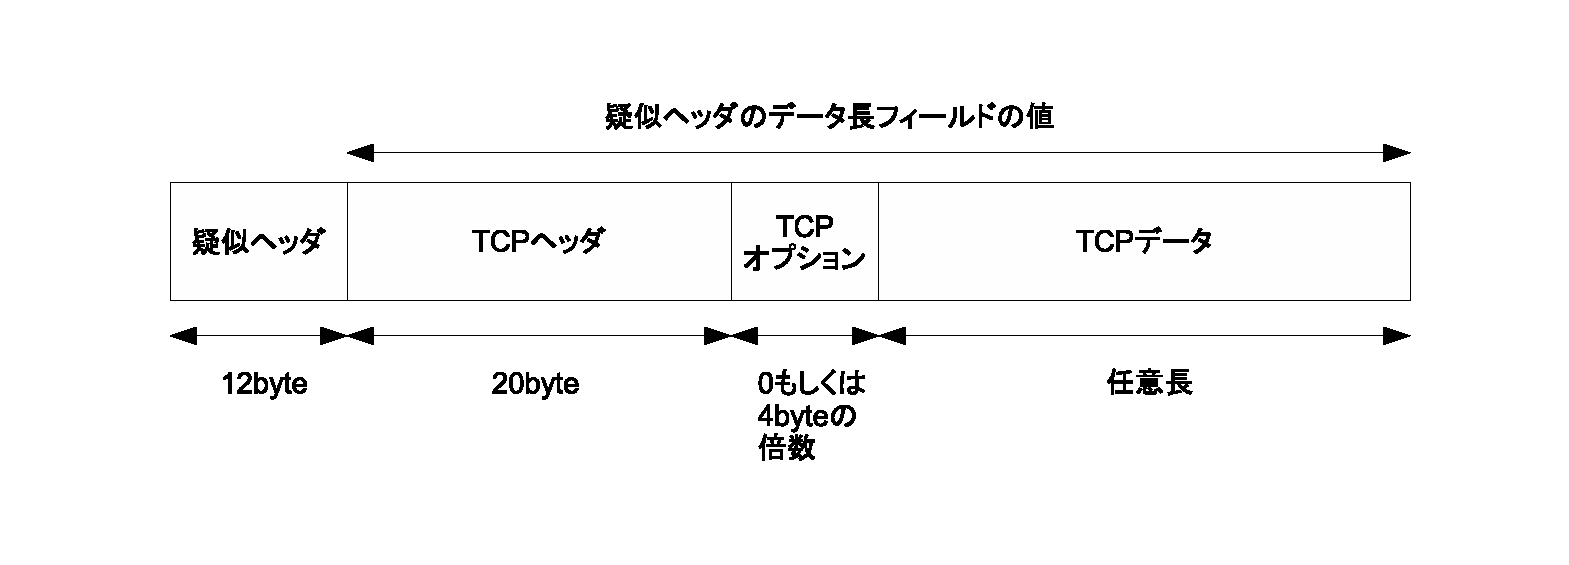
\includegraphics[width=12cm,clip]{draw/tcppseudo.eps}
	\caption{疑似ヘッダを含めたTCPセグメント}
	\label{fig:tcppseudo}
\end{figure}

TCPも、チェックサム計算の際に、TCPヘッダの直前に疑似ヘッダを付加する。TCPヘッダのチェックサムフィールドの値も、TCP疑似ヘッダ込みで計算されたものである。



TCPでは、ヘッダのチェックサムフィールドの計算は必須となる。チェックサムの計算時は、TCPヘッダのチェックサムフィールドは0であると仮定して計算を行う。

IPアドレスの情報を含む疑似ヘッダを用いることで、TCPでも、発信元、宛先の情報を加味して、TCPセグメントの正当性を評価することが可能となる。

